% Created: Enze Chen, June 2017
% Last edited: Enze Chen, February 2018
%
% Chapter 4 of the MSE 142 coursereader. This chapter discusses quantum tunneling using the finite potential step/barrier. It derives the math behind boundary conditions and tunneling probability. Interference from multiple boundaries is also discussed. There is an emphasis on applications to really drive the point home that this phenomenon is cool and more ubiquitous than we might initially think!

% Uncomment the following three lines and last line to individually compile this chapter
%\documentclass[12pt, english]{book}
%\usepackage{142crstyle}
%\begin{document}

\chapter{Quantum Tunneling} \label{ch:tunnel}
%{ \doublespacing 
Imagine you're tossing a tennis ball against the wall. Classical mechanics says that the ball will bounce back at you, or, should you throw it very hard, it might get stuck in the wall. But what if the ball somehow \emph{goes through} the wall and emerges on the other side, leaving both unscathed? This is the basis for \textbf{quantum tunneling}, a phenomenon where a particle passes through a potential barrier that it classically could not surmount. As bizarre as this may seem, quantum mechanics says there is a non-zero probability for tunneling to occur, and this phenomenon is actually leveraged for a variety of physical applications. Tunneling at the quantum scale occurs in physical systems ranging from photons\footnote{See D. D. Coon \href{http://aapt.scitation.org/doi/10.1119/1.1972893}{\emph{American Journal of Physics}} \textbf{34}, 240 (1966).} to water\footnote{See \href{https://physics.aps.org/articles/v9/43}{this focus article} from \emph{Physics} \textbf{9}, 43 about the work of A. I. Kolesnikov et al, \href{https://journals.aps.org/prl/abstract/10.1103/PhysRevLett.116.167802}{\emph{Physical Review Letters}} \textbf{116}, 167802 (2016).} and we will spend this chapter exploring the nature of this truly quantum mechanical behavior.

%%%%%%%%%%%%%%%%%%%%%%%%%%%%%%%%%%%%%%%%%%%%%%%%%%%%%%%%%%%%%%%%%%%%%%%%%%%%%%%%

\section{Finite potential step}
To facilitate our analysis of this behavior, we need to first devise a simple model for a quantum mechanical system, which we have shown here in Figure~\ref{fig:tunnel-step}. On the left half of the figure in region I, where $x < 0$, we have a free particle ($V=0$) traveling to the right with energy $E$. At $x=0$, the particle encounters a \textbf{potential step} with some \emph{finite} potential $V=V_0$ that extends for all $x>0$ into region II.

\begin{figure}[!h]
	\centering
	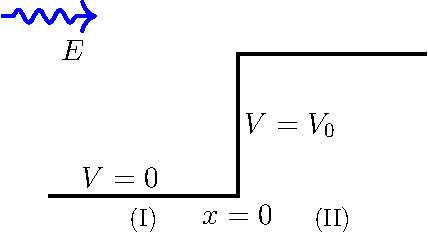
\includegraphics[width=0.42\linewidth]{tunnel-step}
	\caption{A simple model to demonstrate quantum tunneling. A free particle with energy $E$ is traveling to the right and at $x=0$ is incident on a finite potential step with magnitude $V_0$.}
	\label{fig:tunnel-step}
\end{figure}

Note that we have not said anything yet about the relationship between $E$ and $V_0$ (the vertical position of the particle in Figure~\ref{fig:tunnel-step} was arbitrarily drawn). Since the finite potential step is time-independent, we will try to understand how quantum mechanical particles interact with such a potential by solving the time-independent \Sch\ equation. In region I, we only have the free particle, so we can write down the \Sch\ equation as 
\begin{equation}
	-\frac{\hbar^2}{2m} \dv[2]{\Psi}{x} = E\Psi \label{eq:reg-1-se}
\end{equation}
In region II, we have
\begin{equation}
	-\frac{\hbar^2}{2m} \dv[2]{\Psi}{x} = (E-V_0)\Psi \label{eq:reg-2-se}
\end{equation}
where the energy of the particle is now with reference to the step's potential. We've seen these kinds of equations before and know that the general solution are sines and cosines, as was the case with the particle in a box. Here we write the general solutions in a slightly different, but equivalent way:
\begin{tcolorbox}[title = Traveling wave solutions] \vspace{-2ex}
	\begin{align}
		\Psi_{\text{I}} &= Ae^{ik_1x} + Be^{-ik_1x} \label{eq:reg-1-wf} \\
		\Psi_{\text{II}} &= Ce^{ik_2x} + De^{-ik_2x} \label{eq:reg-2-wf} 
	\end{align}
\end{tcolorbox}
where $A$, $B$, $C$, and $D$ are unknown coefficients. Whoa! We know by Euler's formula that complex exponentials can be reformulated as sinusoidal functions, so these solutions at least seem plausible on the surface. To be sure we did our math right, let's plug Equation~\ref{eq:reg-1-wf} into Equation~\ref{eq:reg-1-se} to verify that it is a valid solution.
\begin{align*}
	-\frac{\hbar^2}{2m} \dv[2]{\Psi_{\text{I}}}{x} &= E\Psi_{\text{I}} \\
	-\frac{\hbar^2}{2m} \dv[2]{x}(Ae^{ik_1x} + Be^{-ik_1x}) &= E(Ae^{ik_1x} + Be^{-ik_1x}) \\
	-\frac{\hbar^2}{2m} \dv{x}(Aik_1e^{ik_1x} - Bik_1e^{-ik_1x}) &= E(Ae^{ik_1x} + Be^{-ik_1x}) \\
	\frac{\hbar^2}{2m} \left(Ak_1^2e^{ik_1x} + Bk_1^2e^{-ik_1x}\right) &= E(Ae^{ik_1x} + Be^{-ik_1x}) \\
	k_1^2\left(Ae^{ik_1x} + Be^{-ik_1x}\right) &= \frac{2mE}{\hbar^2}(Ae^{ik_1x} + Be^{-ik_1x})
\end{align*}

So we see that
\begin{equation}
	k_1 = \sqrt{\frac{2mE}{\hbar^2}} \label{eq:reg-1-k}
\end{equation}
which is the same expression we found previously and shows that Equation~\ref{eq:reg-1-wf} is a valid solution. In a similar vein, we see that the magnitude of the wave vector in region II is given by 
\begin{equation}
	k_2 = \sqrt{\frac{2m(E-V_0)}{\hbar^2}} \label{eq:reg-2-k}
\end{equation}

Note that if $E > V_0$, then $k_2$ is real and we have sinusoidal behavior in region II. This makes sense because a particle with higher energy than the potential step should be able to surmount it and continue exhibiting wave-like behavior. However, if $E < V_0$, then $k_2$ becomes imaginary, and the wave-like solutions given in Equation~\ref{eq:reg-2-wf} turn into exponentially growing and decaying functions. Thus it seems like even though the particle does not have sufficient energy to surmount the potential step, there is still something happening in region II \emph{inside} the step. We will come back to this point shortly. \par 

%%%%%%%%%%%%%%%%%%%%%%%%%%%%%%%%%%%%%%%%%%%%%%%%%%%%%%%%%%%%%%%%%%%%%%%%%%%%%%%%

\section{Forward and backward waves}
Now, the general solutions given by Equation~\ref{eq:reg-1-wf} and~\ref{eq:reg-2-wf} are perfectly acceptable mathematically, but we argued in class that there is also a useful physical interpretation of these solutions. Recall that the de Broglie relation relates the wave vector $k$ to the momentum. Now we see that these wave function solutions not only resemble the plane wave solutions that we started with, but they also have a superposition of positive and negative wave vectors which determine the direction of propagation of the wave. We therefore argue that we can associate $A$ with the amplitude of the \textbf{incident wave} on the step (since the exponent has a positive $k_1$) and $B$ with the amplitude of the \textbf{reflected wave} (arising from a reflection at the interface). Similarly, we will associate $C$ with the amplitude of the \textbf{transmitted wave} through the step and $D$ with the amplitude of the wave incident on the step from the right. \par 

In the example shown in Figure~\ref{fig:tunnel-step}, because we are only considering a wave incident on the step from the left, the coefficient $D$ must be zero. For the case when $E > V_0$, we still have a complex exponential function, so the wave function hasn't changed much. But for the case when $E < V_0$, the wave function in region II is only an exponentially damped function, which as we discussed in class is analogous to an evanescent wave in wave optics.\footnote{Indeed, evanescent wave coupling causes \href{https://en.wikipedia.org/wiki/Total_internal_reflection\#Frustrated_total_internal_reflection}{``frustrated'' total internal reflection}, which is a very similar behavior to quantum tunneling.} To see why this is the case, we can define a constant
\begin{equation}
	k' = \sqrt{\frac{2m(V_0-E)}{\hbar^2}} \label{eq:reg-2-kp}
\end{equation}
such that
\begin{equation*}
	k_2 = \sqrt{\frac{2m(E-V_0)}{\hbar^2}} = i\sqrt{\frac{2m(V_0-E)}{\hbar^2}} = ik'
\end{equation*}

This allows us to rewrite Equation~\ref{eq:reg-2-wf} as 
\begin{equation}
	\Psi_{\text{II}} = Ce^{ik_2x} = Ce^{-k'x} \label{eq:reg-2-wfp}
\end{equation}

and the exponential decay function emerges. Our goal now is to extract the reflection coefficient $R$ and transmission coefficient $T$. We define these two quantities as follows:
\begin{equation*}
	\boxed{R = \abs{\frac{B}{A}}^2 \quad \text{and} \quad T = \frac{k_2}{k_1}\abs{\frac{C}{A}}^2}
\end{equation*}
% TODO: check with Aaron about this
Similar to the statistical interpretation of the wave function, we have taken the modulus squared to represent the probability of an event occurring. \par 

%%%%%%%%%%%%%%%%%%%%%%%%%%%%%%%%%%%%%%%%%%%%%%%%%%%%%%%%%%%%%%%%%%%%%%%%%%%%%%%%

\section{Continuity condition}
In order to relate the coefficients from the wave function in region I with those from the wave function in region II, we have to be precise and specify the behavior at the boundary of the two regions (i.e. at $x=0$). Let us consider what the conditions are for continuity of the wave function and its first derivative in a region where the potential is discontinuous (as it is at $x=0$). Starting from the time-independent \Sch\ equation, we integrate over an infinitesimal region $(-\epsilon, \epsilon)$ about $x=0$:
\begin{align*}
	-\frac{\hbar^2}{2m} \dv[2]{\Psi}{x} + V(x)\Psi &= E\Psi \\
	\dv[2]{\Psi}{x} &= \frac{2m}{\hbar^2}(V(x) - E)\Psi \\
	\int_{-\epsilon}^{\epsilon} \dv[2]{\Psi(x)}{x} \dd{x} &= \frac{2m}{\hbar^2} \int_{-\epsilon}^{\epsilon} (V(x)-E)\Psi(x) \dd{x} 
\end{align*}

Now as $\epsilon$ approaches zero, the right hand side approaches zero if $V(x)$ and $\Psi(x)$ are not infinite (and there are good reasons why $\Psi$, from which one calculates the probability density function, cannot go to infinity).\footnote{Though $\Psi(x)$ cannot be infinite at the boundary, $V(x)$ still can. We'll save this for the next chapter when we discuss the Kronig-Penney model.} We therefore conclude, after performing the straightforward integral on the left hand side, that
\begin{tcolorbox}[title = Continuity of the wave function] \vspace{-2ex}
	\begin{equation}
		\dv{\Psi}{x} \bigg|_{\epsilon} - \dv{\Psi}{x} \bigg|_{-\epsilon} = 0 \label{eq:cont-dx}
	\end{equation}
\end{tcolorbox}

This means that across the discontinuity in the potential, the first derivative of the wave function (and by extension the wave function itself) must be continuous.\footnote{Continuity of the wave function is an important point, so if you need another explanation to internalize the ideas, \href{https://www.quora.com/Why-does-the-wave-function-have-to-be-continuous}{Quora} actually gives a pretty good answer.} 

%%%%%%%%%%%%%%%%%%%%%%%%%%%%%%%%%%%%%%%%%%%%%%%%%%%%%%%%%%%%%%%%%%%%%%%%%%%%%%%%

\section{Tunneling probability}
Equation~\ref{eq:cont-dx} allows us to obtain the desired transmission and reflection coefficients as follows. At the boundary, we require that 
\begin{align*}
	\Psi_{\text{I}}(0) &= \Psi_{\text{II}}(0) \\
	\Psi_{\text{I}}'(0) &= \Psi_{\text{II}}'(0)
\end{align*}
which directly translates into
\begin{align}
A + B &= C \label{eq:abc1} \\
Ak_1 - Bk_1 &= Ck_2 \label{eq:abc2}
\end{align}

We can solve the above system of equations in many ways, such as multiplying Equation~\ref{eq:abc1} by $k_1$ and adding the result to Equation~\ref{eq:abc2}. Doing so gives
\begin{equation}
	\frac{C}{A} = \frac{2k_1}{k_1+k_2} \label{eq:c-a}
\end{equation}
and a similar method gives 
\begin{equation}
	\frac{B}{A} = \frac{k_1 - k_2}{k_1 + k_2} \label{eq:b-a}
\end{equation}

Finally, this gives 
\begin{tcolorbox}[title = $T$ and $R$ for finite potential step] \vspace{-2ex}
	\begin{align}
		T = \frac{k_2}{k_1}\abs{\frac{C}{A}}^2 &= \frac{4k_1k_2}{(k_1+k_2)^2} \label{eq:t-step} \\ 
		R = \abs{\frac{B}{A}}^2 &= \frac{(k_1-k_2)^2}{(k_1+k_2)^2} \label{eq:r-step}
	\end{align}
\end{tcolorbox}
If you have taken a course in optics or acoustics these equations should look familiar---they are similar to the results for the transmission and reflection coefficients for an acoustic wave or light wave incident on a boundary. Now we're beginning to see how quantum mechanics predicts transmission with a non-zero probability. Note here that the way we have defined $T$ and $R$ also gives us the identity $T + R = 1$. \par 

%%%%%%%%%%%%%%%%%%%%%%%%%%%%%%%%%%%%%%%%%%%%%%%%%%%%%%%%%%%%%%%%%%%%%%%%%%%%%%%%

\section{Finite potential barrier} \label{sec:tunnel-barrier}
Having successfully managed the previous example, we're now ready to tackle the slightly more complicated case (and the one that we've been waiting for!) of quantum tunneling through a finite potential barrier of width $L$ and height $V_0$ (Figure~\ref{fig:tunnel-barrier}). We will carry out the following calculations in particular for the case $E < V_0$, which is the most interesting and surprising case.

\begin{figure}[!h]
	\centering
	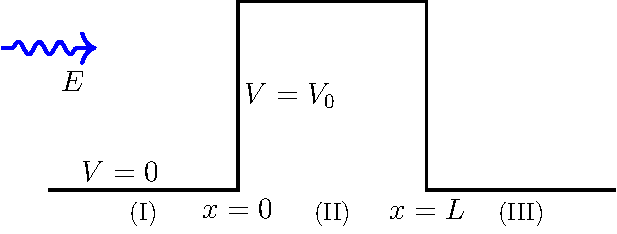
\includegraphics[width=0.6\linewidth]{tunnel-barrier}
	\caption{In this example, a free particle with energy $E$ is traveling to the right and at $x=0$ is incident on a finite potential barrier with width $L$ and height $V_0$. The potential is otherwise zero in front of and behind the barrier.}
	\label{fig:tunnel-barrier}
\end{figure}

With three regions, we can now write down the solutions to the time-independent \Sch\ equation as
\begin{align}
	\Psi_{\text{I}} &= Ae^{ikx} + Be^{-ikx} \label{eq:barr-1} \\
	\Psi_{\text{II}} &= Ce^{k'x} + De^{-k'x} \label{eq:barr-2} \\
	\Psi_{\text{III}} &= Fe^{ikx} \label{eq:barr-3}
\end{align}

Here, we have defined $k = \sqrt{\frac{2m}{\hbar^2}(E)}$ and $k'=\sqrt{\frac{2m}{\hbar^2}(V_0-E)}$ such that $k'$ is a real number. As before, we note that Equation~\ref{eq:barr-2} models exponential growth and decay inside the barrier. We also argue that a particle incident only from the left means that the only term in region III is the transmitted wave with amplitude $F$ (Equation~\ref{eq:barr-3}). Now our goal is to extract the transmission coefficient $T = \abs{\frac{F}{A}}^2$.\footnote{Whereas previously we had an extra $k_2/k_1$ term, in this case the momentum of the wave in region I and region III are the same! It might seem weird, but tunneling doesn't cause the wave to actually lose energy.} In this case, the transmitted wave with amplitude $F$ encodes within it all the possible ways in which the wave can transmit through the barrier, including multiple reflections inside the barrier. All of these complicated possibilities are accounted for simply by enforcing the continuity equations at $x=0$ and $x=L$. This gives us the following set of equations:
\begin{align*}
	A + B &= C + D \\
	A - B &= (C - D)\frac{k'}{ik} \\
	Ce^{k'L} + De^{k'L} &= Fe^{ikL} \\
	Ce^{k'L} - De^{k'L} &= Fe^{ikL}\frac{ik}{k'}
\end{align*}

We will not go through the gory details here of solving this system of equations as it involves messy algebra and nothing more of substance, but feel free to consult Appendix~\ref{sec:tunnel-deriv} for all the steps. After combining these equations and eliminating variables appropriately, we obtain the following equation relating $F$ to $A$:
\begin{equation}
	4Aikk'e^{-ikL} = F \left[(k'+ik)^2e^{-k'L} - (k'-ik)^2e^{k'L}\right] \label{eq:tunnel-fa}
\end{equation}

In the limit where $k'L \gg 1$ (i.e. the barrier width is much larger than the effective wavelength of the particle inside the barrier), one can simplify Equation~\ref{eq:tunnel-fa} to obtain
\begin{equation}
	T = \abs{\frac{F}{A}}^2 = \frac{16k^2k^{\prime 2}e^{-2k'L}}{(k^{\prime 2}+k^2)^2} \label{eq:tunnel-prob}
\end{equation}

Since this expression for $T$ is dominated by the exponential term, it asymptotically approaches the very simple equation
\begin{tcolorbox}[title = Tunneling probability approximation when $E < V_0$] \vspace{-2ex}
	\begin{equation}
		T \approx e^{-2k'L} \label{eq:tunnel-approx}
	\end{equation}
\end{tcolorbox}

The above equation is a very useful approximate solution for the tunneling probability that is often applied in practice. For completeness, we will also give the exact solution for the tunneling probability below.
\begin{tcolorbox}[title = Tunneling probability exact solution when $E < V_0$] \vspace{-2ex}
	\begin{equation}
		T = \abs{\frac{F}{A}}^2 = \frac{1}{1 + \left(\frac{k^2+k^{\prime 2}}{2kk'}\right)^2 \sinh^2(k'L)} \label{eq:tunnel-prob-full}
	\end{equation}
\end{tcolorbox}

The exact solution has a maximum value of 1 when $k'L=0$ and rapidly decreases to 0 as $k'L$ increases. However, $T$ is still non-zero, which means there is a chance for the particle to tunnel through the barrier and emerge on the other side! This is shown schematically in Figure~\ref{fig:tunnel-wave}.\footnote{What we've plotted is the actual wave function amplitude. How would the probability density differ?} As discussed in class, for $L \approx \SI{1}{\nano\meter}$ and for typical electron-volt-scale potential barriers, the transmission probability is close to 1, indicating how important these kinds of effects become at the nanoscale. \par

\begin{figure}[!h]
	\centering
	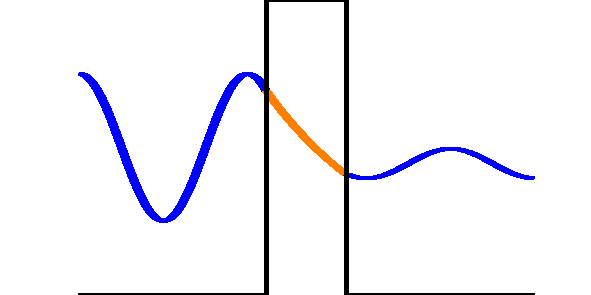
\includegraphics[width=0.48\linewidth]{tunnel-wave}
	\caption{An illustration of the amplitude of the wave function in the three regions. It exponentially decays through the barrier but emerges from the right side with a lower amplitude and the same frequency (energy) as the wave function in the left region. A non-zero value of the wave function on the right indicates that the particle may exist past the barrier.}
	\label{fig:tunnel-wave}
\end{figure}

Furthermore, note how the wave function in region III differs from the wave function in region I. The amplitude is much smaller, which makes sense as there is a much lower probability that we will find the particle on the right side of the barrier. However, should tunneling occur, we can apply the conservation of energy to see that the particle has the same energy as before, and hence the frequency of the wave function is the same. It's easy to get probability and energy mixed up, but make sure you can draw the distinction.\footnote{An analogy to classical mechanics: A ball with a certain amount of kinetic energy that rolls up and over a hill will have the same amount of kinetic energy when it arrives back to ground level (assuming no friction).} \par 

Though we did not derive it here, it is interesting to look at the transmission probability for the case when $E > V_0$, which is given by Equation~\ref{eq:tunnel-prob-res} and plotted in Figure~\ref{fig:tunnel-prob} as a function of energy.
\begin{equation}
	\boxed{T = \frac{1}{1 + \left(\frac{k^2-k_2^2}{2kk_2}\right)^2 \sin^2(k_2L)}} \label{eq:tunnel-prob-res}
\end{equation}

\begin{figure}[!h]
	\centering
	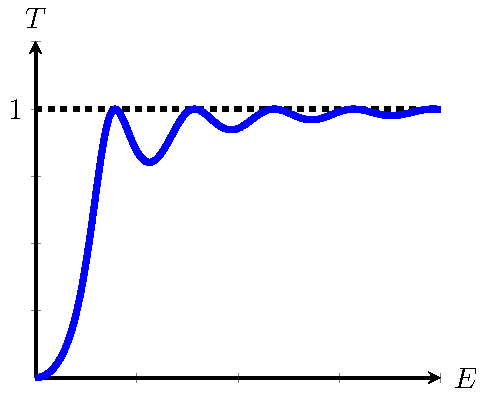
\includegraphics[width=0.35\linewidth]{tunnel-prob}
	\caption{Tunneling probability as a function of energy for the finite potential barrier when $E > V_0$. At characteristic energies, the tunneling probability reaches 1 due to resonance of the wave function in the region of the barrier.}
	\label{fig:tunnel-prob}
\end{figure}

In this case, the wave function displays sinusoidal behavior in region II instead of exponential behavior, and we have made the appropriate substitution as $k_2=ik'$. It may come as no surprise that if the energy of the particle was high enough, then the transmission probability approaches 1 (i.e. it's as if the barrier wasn't even there). However, as seen in Figure~\ref{fig:tunnel-prob}, total transmission is also achievable at lower values of $E$, which correspond to tunneling \textbf{resonance} when the wavelength of the particle coincides with the width of the barrier. This leads to a constructive interference effect analogous to what we observed in the double-slit experiment.

%%%%%%%%%%%%%%%%%%%%%%%%%%%%%%%%%%%%%%%%%%%%%%%%%%%%%%%%%%%%%%%%%%%%%%%%%%%%%%%%

\section[Application: Devices]{Application: Optical and electronic devices}
Once the theory behind quantum tunneling was formally developed, scientists suddenly realized just how ubiquitous the phenomenon was. It turns out quantum tunneling is necessary to explain the radioactive decay of nuclei, the fusion reactions inside stars, and even the mechanisms behind photosynthesis! Furthermore, scientists have leveraged quantum tunneling to create many new nanoscale devices, two of which will be discussed here.

\subsection{Quantum cascade laser}
The first device we will survey here, the \textbf{quantum cascade laser} (QCL), actually combines quantum tunneling with the quantum wells that we analyzed in the previous chapter. First demonstrated in 1994 using a mixture of GaInAs/AlInAs, QCLs are semi-conductor lasers comprised of a stack of quantum well heterostructures (Figure~\ref{fig:qcl}).

\begin{figure}[!h]
	\centering
	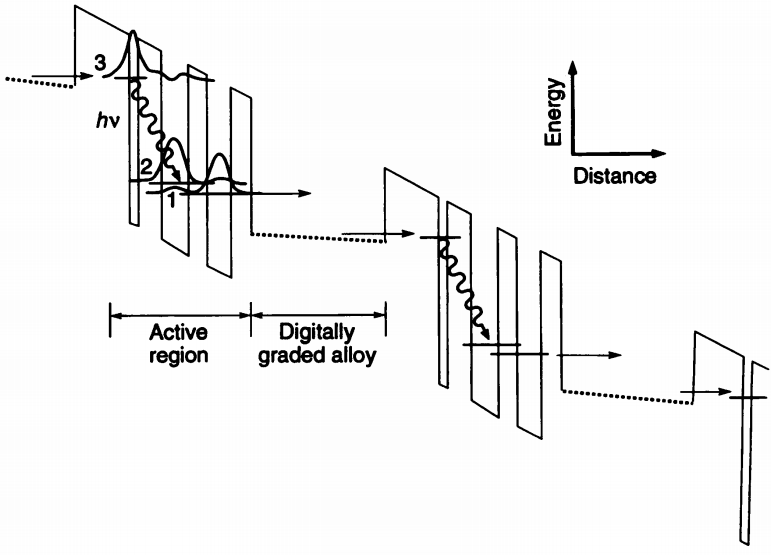
\includegraphics[width=0.55\linewidth]{qcl}
	\caption{Schematic of the quantum cascade laser, where periodic layers of varying thicknesses confine electrons into different energy levels. A population inversion causes electron transitions that lead to photon emission and subsequent tunneling of the electron to the next period in the structure. Reproduced from J. Faist et al. \href{http://science.sciencemag.org/content/264/5158/553}{\emph{Science}} \textbf{264}, 5158 (1994).}
	\label{fig:qcl}
\end{figure}

Instead of having a bulk structure, QCLs use a periodic series of layers of different materials and thicknesses to achieve a superlattice. This superlattice is capable of confining electrons into different discrete sub-bands across all of the quantum wells. When a \textbf{population inversion} is achieved, where more electrons are in an excited state than in the ground state, electrons will drop in energy and emit photons, which is how all lasers operate in general. What makes the QCL unique, in addition to its highly tunable layers (e.g. grown with molecular beam epitaxy), is that once an electron has transitioned to a lower energy level in one period of the structure, it can then tunnel to the next period in the heterostructure and undergo more transitions, thereby releasing more photons in a \emph{cascading} effect. The ability for electrons to tunnel through barriers and emit multiple photons leads to higher power output for QCLs than normal lasers, which could lead to advances in spectroscopy, sensing, and signaling.

%%%%%%%%%%%%%%%%%%%%%%%%%%%%%%%%%%%%%%%%%%%%%%%%%%%%%%%%%%%%%%%%%%%%%%%%%%%%%%%%

\subsection{Scanning tunneling microscope}
Our second nanoscale device, the \textbf{scanning tunneling microscope} (STM), is a more popular tool that you might have previously heard about. It was developed in 1981 by Gerd Binnig and Heinrich Rohrer at IBM, and a schematic detailing the principles of operation is shown in Figure~\ref{fig:stm}.

\begin{figure}[!h]
	\centering
	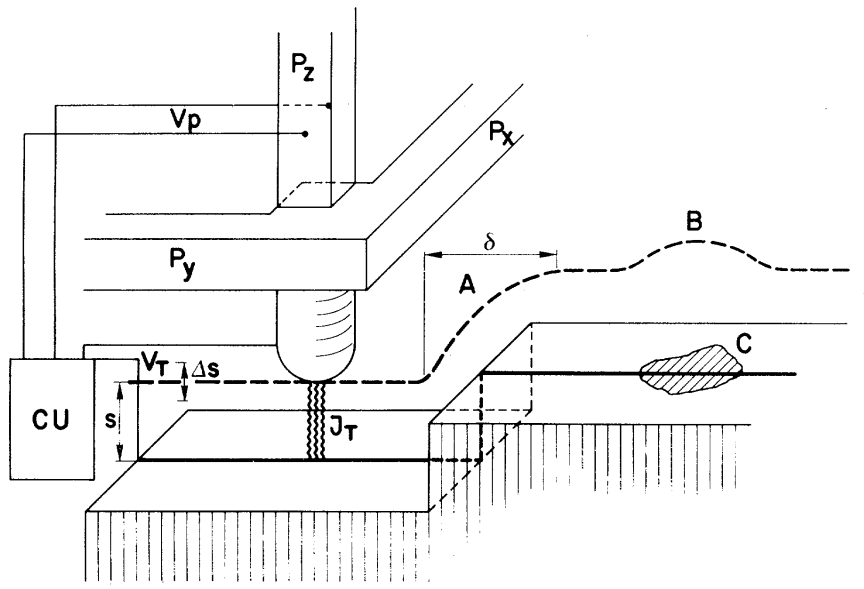
\includegraphics[width=0.5\linewidth]{stm}
	\caption{Schematic for how the scanning tunneling microscope operates. As the tip moves across the surface, the control unit (CU) applies an appropriate voltage $V_p$ to a piezoelectric arm $P_z$ and modulates its height such that the same tunneling current $J_T$ is maintained. As a result, the tip moves up and down to trace a material's topography, which is imaged at angstrom-scale resolution. Reproduced from G. Binnig et al. \href{https://journals.aps.org/prl/abstract/10.1103/PhysRevLett.49.57}{\emph{Phys. Rev. Lett.}} \textbf{49}, 57 (1982).}
	\label{fig:stm}
\end{figure}

In order to detect small changes on a material's surface, the STM leverages \textbf{piezoelectricity} to control the three arms that guide a sharp tip that sits less than \SI{1}{\nano\meter} away from the surface.\footnote{For those unfamiliar with piezoelectricity, it is briefly explained by \href{http://hyperphysics.phy-astr.gsu.edu/hbase/Solids/piezo.html}{Rod Nave} at Georgia State University.} As $P_x$ and $P_y$ raster scan the tip across the surface, a control unit applies a small voltage ($\sim\SI{10}{\milli\volt}$) to cause electrons to tunnel between the tip and the surface. It measures the tunneling current $J_T$ that's produced and adjusts the height of the third arm $P_z$ to maintain the same current. The piezoelectric arms are so sensitive to changes in $J_T$ that the STM is capable of imaging the surface topography with a resolution of \SI{1}{\angstrom} (\SI{e-10}{\meter}) or less! Not only are scientists able to image \emph{individual atoms} with this technique, but they have been able to manipulate the atoms as well, forming unique nanostructures like the quantum corral in Figure~\ref{fig:corral} and even a stop-motion animated short film by the folks at IBM Research.\footnote{A video of ``A Boy and His Atom'' and more information can be found on the \href{http://www.research.ibm.com/articles/madewithatoms.shtml\#fbid=9xTkVKSpT3k}{IBM Research website}.}

\begin{figure}[!h]
	\centering
	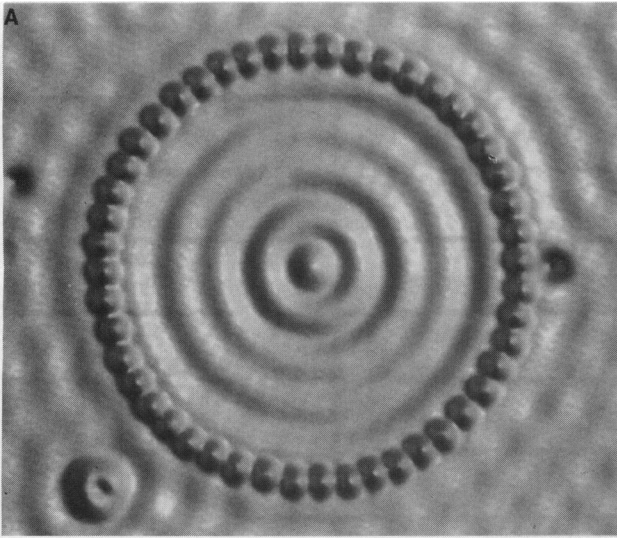
\includegraphics[width=0.4\linewidth]{corral}
	\caption{A quantum corral constructed by arranging 48 Fe atoms in a ring on Cu(111) surface using a STM. Reproduced from M. F. Crommie et al. \href{http://science.sciencemag.org/content/262/5131/218}{\emph{Science}} \textbf{262}, 5131 (1993).}
	\label{fig:corral}
\end{figure}

%%%%%%%%%%%%%%%%%%%%%%%%%%%%%%%%%%%%%%%%%%%%%%%%%%%%%%%%%%%%%%%%%%%%%%%%%%%%%%%%

%\subsection{Resonant tunneling diode}

%%%%%%%%%%%%%%%%%%%%%%%%%%%%%%%%%%%%%%%%%%%%%%%%%%%%%%%%%%%%%%%%%%%%%%%%%%%%%%%%

\section{Summary}
To recap, in this chapter we analyzed the peculiar phenomenon of quantum tunneling, whereby a particle incident on a finite potential barrier has a non-zero probability of penetrating the barrier and emerging on the other side. This holds true even if the particle carried less energy than the barrier's potential, which is prohibited by the laws of classical mechanics. In that case, we argued that the wave function of the particle exhibits exponential behavior inside the barrier and it must maintain continuity with the wave function on the outside. This allowed us to derive the transmission probability as a function of the particle's wave vector and the barrier width, and we typically use Equation~\ref{eq:tunnel-approx} to approximate this probability. Tunneling is a vital mechanism for many natural processes and scientists have leveraged its power to create novel nanoscale devices like the quantum cascade laser and scanning tunneling microscope. In the next chapter, we will solve the \Sch\ equation for yet another model, one that consists of periodic potential barriers that are infinitely tall and infinitely narrow.


%} % for doublespacing
%\end{document}